\section{Problem formulation}
\label{sec:ocpl_problem}
As described in Section \ref{sec:occp_related_works}, this thesis primarily addresses the problem of Visual-Conditioned Multi-Task Imitation Learning. The goal is to train a single conditioned control function, $\pi_{\theta}(a_{t}| o^{a}_{t}, c_m)$, that can guide a robotic agent in solving both variations of a given task and entirely different tasks. Where, the input consists of a command $c_m$, represented as a video demonstration of the requested task, along with the current observation of the agent $o^{a}_{t}$.

The approach proposed in this thesis is based on the observation that solving this problem involves two key tasks:
\begin{itemize}
    \item \textit{Command analysis}: This task involves solving a cognitive problem, where the system must interpret the high-level task command, understand the task intent, identify the relevant objects, and recognize the required actions.
    \item \textit{Action generation}: This task involves solving a control problem, where the system must correlate the information from the command analysis with the agent environmental state to generate a valid action that moves the robot toward completing the requested task.
\end{itemize}

As demonstrated in the comprehensive review of related works (Section \ref{sec:occp_related_works}), the Visual-Conditioned MTIL problem is typically addressed using end-to-end architectures, which are trained with an action-centric behavioral cloning loss. While these systems are often able to control the robot and produce \textbf{reasonable trajectories} to complete tasks like pick-and-place, they may manipulate the wrong object, indicating a limitation in the cognitive ability to correctly identify the relevant object.


In this thesis, a modular approach is adopted. Specifically, Figure \ref{fig:end_to_end_vs_modular} illustrates the differences between a general end-to-end architecture and the proposed modular architecture. In the end-to-end architecture, the \textit{Backbone Module}, which can be any deep learning architecture used in state-of-the-art methods, takes both the agent observation $o^{a}_t$ and the command $c_{m_i}$ as input. It generates an embedding $z_t$ that must encapsulate all the necessary information for the \textit{Control Module} to produce a valid action. This includes details derived from both the command, such as the position of the object of interest, the task being solved, its variations, as well as the state of the agent itself.

In contrast, the modular approach utilizes two backbone modules. The first, the \textit{Command Analysis Backbone}, explicitly solves the cognitive task, producing task-relevant information ($z^{task}_t$) such as the position of the object of interest. The second, the \textit{Control Backbone Module}, generates a control embedding ($z^{control}_t$), which directly encodes information relevant to the action to be performed. In this modular approach, the \textit{Control Module} takes both the task-relevant information ($z^{task}_t$) and the control embedding ($z^{control}_t$) as inputs.

\begin{figure}[t]
    \centering
    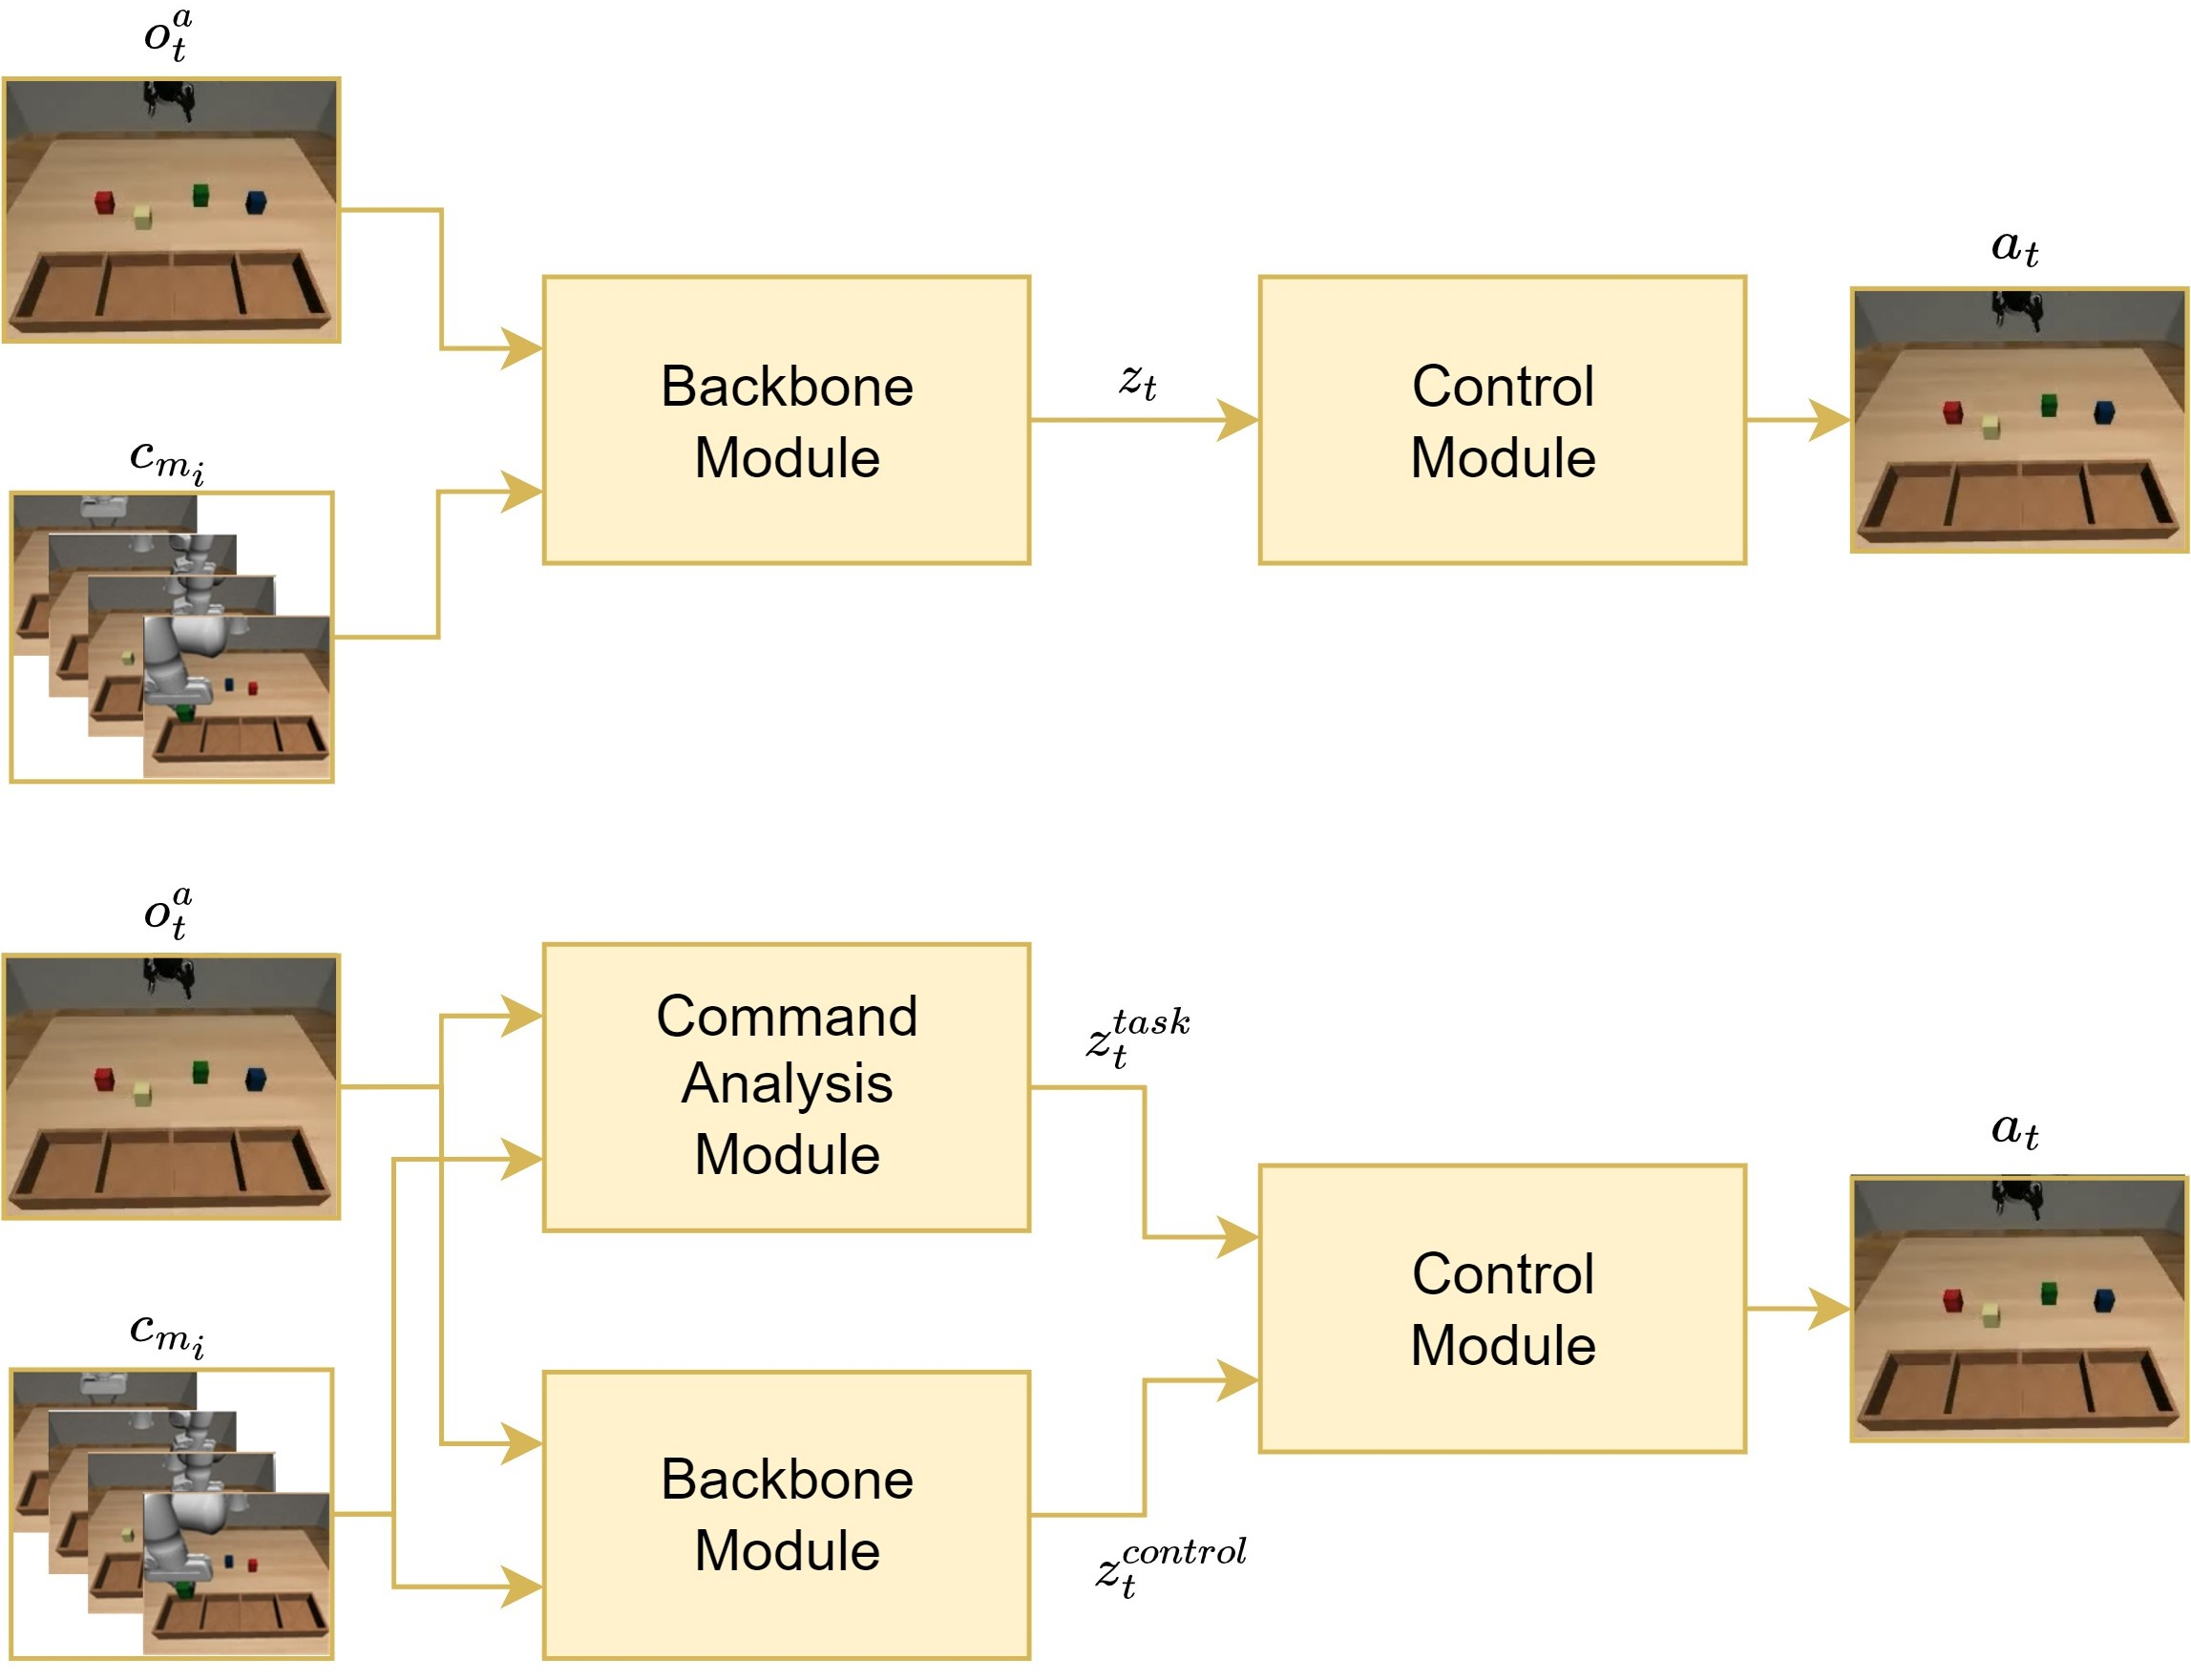
\includegraphics[width=0.7\textwidth]{figures/images/ch3/end_to_end_vs_modular.jpg}
    \caption{(Upper) General end-to-end architecture, where the \textit{Backbone Module} takes as input both the agent observation and the command. It generates an embedding $z_{t}$ that must contain information related to both the command and the control. (Bottom) In the modular architecture, there are two backbone modules: the \textit{Command Analysis Module}, which generates the task-embedding $z^{task}_t$, and the \textit{Backbone Module}, which is trained to generate only the control-embedding $z^{control}_{t}$.}
    \label{fig:end_to_end_vs_modular}
\end{figure}


The underlying assumption of this approach is that by separating the problem into two components, cognitive and control, and designing task-specific modules trained independently of each other, the system becomes more robust. For example, the Command Analysis Module is trained specifically for the cognitive task (e.g., the Conditioned Object Detection task described in Chapter \ref{ch:cod}), while the Control Backbone is trained for the control task. This separation allows the final Control Module to be informed by optimal embeddings generated by modules trained on task-specific problems.

Section \ref{sec:} provides an example of a cognitive problem that can be addressed by the Command Analysis Backbone. Here, the focus is on describing the problem solved in order to learn the final control policy $\pi_{\theta}$. Specifically, the goal is to learn the parameters of the policy $\pi_{\theta}$ using a supervised-learning approach.

The first step is defining the dataset. As explained in Section \ref{sec:bc}, in multi-task, multi-variation scenario, there are $n$ distinct tasks, denoted by $\mathcal{T} = \left\{T_{1}, T_{2}, \dots, T_{n}\right\}$, where each task $T_{i}$ is associated with a set of variations $\mathcal{M}_{i}$. For each task, a specific dataset $\mathcal{D}_{i} = ((c_{m}, \tau_{m}), m \in \mathcal{M}_{i})$ is constructed, containing pairs of demonstrator videos $c_{m}$ and corresponding target trajectories $\tau_{m}$ for each variation. The demonstrator video consists solely of visual observations, represented as $c_{m} = \left\{o^{d}_{1}, o^{d}_{2}, \dots, o^{d}_{T'}\right\}$, while the target trajectory includes both observations and associated actions: $\tau_{m} = \left\{(o^{a}_{1},a_{1}), \dots, (o^{a}_{T}, a_{T})\right\}$.

Building upon the complete dataset $\mathcal{D} = \left\{\mathcal{D}_{1}, \dots, \mathcal{D}_{n}\right\}$, the optimal parameters $\theta^{*}$ are obtained by solving the minimization problem described in Formula \ref{eq:minimization_prob}, where the loss function $\mathcal{L}$ is minimized.
\begin{equation}
    \label{eq:minimization_prob}
    \theta^{*} = \underset{\theta}{\text{arg} \ \min} \ \mathcal{L}(\pi_{\theta}, \mathcal{D})
\end{equation}

Section \ref{sec:ocpl_architecture} will present the specific instance of the proposed architecture, along with the loss function and modules used. The results of the experiments will be discussed in Section \ref{sec:ocpl_experimental}.
